\documentclass[tikz,border=2pt]{standalone}
\usepackage{amsmath,amssymb}
\usetikzlibrary{arrows.meta,decorations.pathreplacing}
\begin{document}
% Compound distribution as a two-stage experiment: first the count N = n with probability P(N=n),
% then a sum of n i.i.d. severities with law F_X^{*n}; F_S mixes these laws with weights P(N=n).
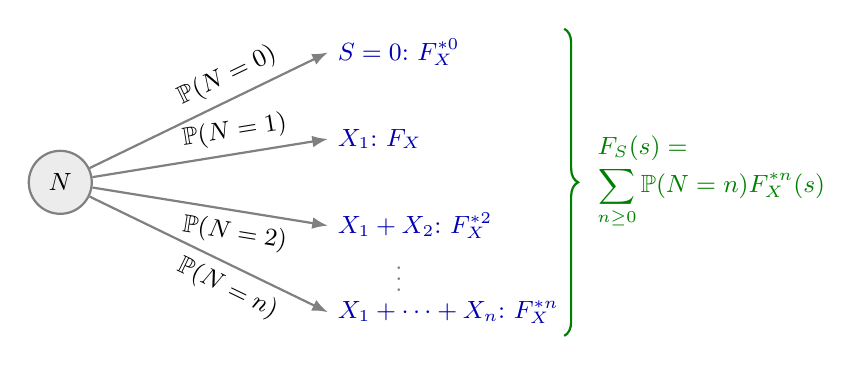
\begin{tikzpicture}[font=\small, >={Latex[length=2mm]}]
  \node[circle, draw=gray, thick, fill=gray!15, minimum size=8mm] (r) at (0,0) {$N$};
  \node[anchor=west, blue!70!black] (l0) at (3.4,1.65) {$S=0$:\ $F_X^{*0}$};
  \node[anchor=west, blue!70!black] (l1) at (3.4,0.55) {$X_1$:\ $F_X$};
  \node[anchor=west, blue!70!black] (l2) at (3.4,-0.55) {$X_1+X_2$:\ $F_X^{*2}$};
  \node[anchor=west, blue!70!black] (l3) at (3.4,-1.65) {$X_1+\dots+X_n$:\ $F_X^{*n}$};
  \draw[->, thick, gray] (r) -- node[pos=0.62, above, sloped, black] {$\mathbb P(N=0)$} (l0.west);
  \draw[->, thick, gray] (r) -- node[pos=0.62, above, sloped, black] {$\mathbb P(N=1)$} (l1.west);
  \draw[->, thick, gray] (r) -- node[pos=0.62, below, sloped, black] {$\mathbb P(N=2)$} (l2.west);
  \draw[->, thick, gray] (r) -- node[pos=0.62, below, sloped, black] {$\mathbb P(N=n)$} (l3.west);
  \node[gray] at (4.3,-1.12) {$\vdots$};
  \draw[green!50!black, thick, decorate, decoration={brace, amplitude=5pt}] (6.4,1.95) -- (6.4,-1.95);
  \node[green!50!black, anchor=west, align=left] (fs) at (6.7,0) {$F_S(s)=$\\[1pt]$\displaystyle\sum_{n\ge0}\mathbb P(N=n)F_X^{*n}(s)$};
\end{tikzpicture}
\end{document}
